
\chapter[Método da Decomposição]{Método da Decomposição de Adomian}

\section{Introdução}

   O Método da Decomposição de Adomian (ADM) não é uma técnica muito famosa em geral, mas é extremamente poderosa para solucionar equações diferenciais lineares ou não-lineares de diversos tipos. Tal método já foi utilizado com sucesso em diferentes estudos ao longo dos anos, dentre eles podemos citar o trabalho de Mustapha Azreg-Aïnou's - Developed Adomian method for quadratic Kaluza-Klein relativity, e de Antonio Gourlat e Bodmann -An analytical solution for the nonlinear energy spectrum equation by the decomposition method.
   
    De acordo com \apud{schneider}{Adriana}, o Método da Decomposição de Adomian foi apresentado pelo  matemático americano George Adomian (1922-1996) na década de 80. Tal método consiste em separar a equação em duas partes, a parte linear e a não-linear e em sequência aplicar o operador inverso. De acordo com Goulart et.al(2013) as soluções das equações são calculadas como séries infinitas e cada termo dessas séries é um polinômio generalizado chamado polinômio de Adomian.

    
   Em seu livro, Adomian (1956) afirma que o maior objetivo desse método é tornar viável soluções realistas de sistemas complexos sem a obrigação de utilizar-se da modelagem usual.
   
  Segundo Adomian (1988), a diferença é que o Método da Decomposição de Adomian pode fornecer aproximação analítica sem linearização, pertubação, aproximações de fechamento, ou métodos de discretização que podem resultar em complexos modelos computacionais.
   ``Além disso, ao contrário da maioria dos métodos númericos, o Método da Decomposição de Adomian fornece uma forma fechada da solução'' \apud{Dehghan}{Adriana}, ou seja, é capaz de ser representada analiticamente em termos de uma quantidade limitada de funções conhecidas.

  
   

\section{Descrição do Método} 
 
 
 Considerando a seguinte equação diferencial não-linear abaixo
 
 \begin{equation}  \textbf{L}y +  \textbf{R}y +  \textbf{N}y = g\end{equation},

O termo \textbf{L} é o operador derivativo de maior grau da equação, \textbf{R}y representa o termo linear, \textbf{N}y o termo não- linear e \textbf{g} a condição inicial. Resolvendo para \textbf{L}y  e aplicando o operador inversor $L^{-1}$ , têm-se

 \begin{equation}  \textbf{L}y =  g - \textbf{R}y - \textbf{N}y,\end{equation},
 
  
  \begin{equation}
L^{-1}Ly =  L^{-1}g -  L^{-1}Ry -  L^{-1}Ny,
  \end{equation}
  
  L é definido como $\frac{d^ny }{d x^n}$ , sendo assim, $L^{-1}$ é um operador integral de 0 até x,
  \begin{equation}
  L^{-1}= \int_0^{x} (...) dt.
  \end{equation}
  
  Caso L seja de segunda-ordem, $\frac{d^2y}{d x^2}$ por exemplo, $L^{-1}$ será um operador de integração duplo . E a equação se resultará em
  
  \begin{equation}
  y= y(0) + xy'(0) + L^{-1}g - L^{-1}Ry - L^{-1}Ny,
  \end{equation}

Analisando a equação é possível perceber que y(0), xy'(0) são as condições iniciais e $L^{-1}g$ o valor inicial conhecido. Então, $y_{0}$ se resume nos três primeiros termos do lado direito da equação. Também é possível perceber que a parte linear da equação são os termos $y(0)$, $xy'(0)$, $L^{-1}g$ e $L^{-1}Ry$ e sua decomposição é $\sum_{n=0}^{\infty} y_{n}$. Já  o último termo $L^{-1}Ny$ é a parte não-linear, decompondo-o têm-se $\sum_{n=0}^{\infty} A_{n}(y_{0},y_{1},...y_{n})$. Com essas considerações, a equação final se resulta em
 
 \begin{equation}
 \sum_{n=0}^{\infty} y_{n} = y_{0} - L^{-1}R \sum_{n=0}^{\infty} y_{n} - L^{-1}\sum_{n=0}^{\infty} A_{n}.
 \end{equation}
 
 Consequentemente, é possível escrever
 
 \begin{equation}
 y_{1} = -L^{-1} (Ry_{0}) - L^{-1}(A_{0}), \end{equation}
 
 \begin{equation}y_{2} = -L^{-1} (Ry_{1}) - L^{-1}(A_{1}),\end{equation}
 
 \begin{equation}y_{3} = -L^{-1} (Ry_{2}) - L^{-1}(A_{2}),
 \end{equation}
 
 Generalizando para o $y_{n}$ acha-se:
 
 \begin{equation}y_{n} = -L^{-1} (Ry_{n-1}) - L^{-1}(A_{n-1}).
 \end{equation}
 
  De acordo com GOULART et.al (2013) os polinômios de Adomian An são obtidos a partir da expansão da série de Taylor do termo não-linear em torno do primeiro termo da série $y_{0}$. Dependem apenas de $y_{0}$ à $y_{n}$:
  
  \begin{equation}
  A_{0} = f(y_{0}),
  \end{equation}
  
   \begin{equation}
  A_{1} = y_{1}\left(\dfrac{\partial }{\partial y_{0}}\right) f(y_{0}),
  \end{equation}
  
  \begin{equation}
  A_{2} = y_{2} \left(\dfrac{\partial }{\partial y_{0}}\right)f(y_{0}) +\left(\dfrac{y_{1}^2}{2!}\right)\left(\dfrac{\partial^2 }{\partial y_{0}^2}\right)f(y_{0}),
  \end{equation}
 
   \begin{equation}
  A_{3} = y_{3} \left(\dfrac{\partial }{\partial y_{0}}\right)f(y_{0}) + y_{1}y_{2}\left(\dfrac{\partial^2 }{\partial y_{0}^2}\right)f(y_{0}) + \left(\dfrac{y_{1}^3}{3!}\right)\left(\dfrac{\partial^3 }{\partial y_{0}^3}\right)f(y_{0}),
  \end{equation}
  
 \begin{gather*}
 ...
 \end{gather*}
 
 \begin{equation}
  A_{n} = \dfrac{1}{n!} \sum_{v=1}^{n} c(v,n)\left(\dfrac{\partial^vf }{\partial y^v}\right).
 \end{equation}
  
  Quando a equação é linear, f(y) = y , o termo $A_{n}$ reduz para $y_{n}$. Quando a equação é não-linear, $A_{n} = A_{n} (y_{0}, y_{1},...,y_{n})$. Por exemplo $f(y) = y^3$, $A_{0} = y_{0}^3$, $A_{1} = 3y_{0}y_{1}$, $A_{2} = y1^2+3y_{0}y_{2}$, $A_{3} = 3y_{1}y_{2} + 3y_{0}y_{3}$.

 
 
 \section{Exemplos}
 
 Com o objetivo de simplificar o entendimento do Método de Decomposição de Adomian , alguns exemplos de fácil compreensão serão demonstrados a seguir.
 
 \subsection{Exemplo 1 : Equação linear de primeira ordem}
 
 Considere a equacão linear abaixo com a condição linear y(0) = 1:
 
 \begin{gather*}
 y' = y, 
  \end{gather*}
   \begin{gather*}
 \frac{d y}{d x} = y,
 \end{gather*}

Pode-se escrever

\begin{gather*}
 \textbf{L}y - \textbf{R}y = g,
  \end{gather*}
  \begin{gather*}
 \textbf{L}y = 1 + \textbf{R}y ,
  \end{gather*}
  
  Lembrando que L é o operador derivativo de maior ordem, que nesse caso é $\frac{d y}{d x}$, portanto o operador inverso é $L^{-1}=\int_0^{x}\frac{d y}{d x} dx$. Aplicando o operador inverso nos termos da equação, obtêm-se:

\begin{gather*}
 \textbf{L}^{-1}\left(\frac{d y}{d x}\right) = \textbf{L}^{-1} y,
  \end{gather*}
  
  \begin{gather*}
  \int_0^{x}\frac{d y}{d x}dx = \textbf{L}^{-1} y,
\end{gather*} 

Integrando o lado esquerdo,

 \begin{gather*}
  y(x) - y(0) = \textbf{L}^{-1} y,
\end{gather*} 

 \begin{gather*}
  y(x) = y(0) + \textbf{L}^{-1} y,
\end{gather*} 
 
 De acordo com a equação (2.6) obtêm-se:
 
  \begin{gather*}
  y_{0} +y_{1} + y_{2} + ... + y_{n}  = y(0) + \textbf{L}^{-1}( y_{0} +y_{1} + y_{2} + ... + y_{n}).
\end{gather*}

É importante notar que nesse exemplo não serão utilizados os polinômios de Adomian $A_{n}$  devido ao fato da equação ser inteiramente linear.
A partir deste momento basta comparar o lado esquerdo da equação acima com o lado direito da mesma e aplicar o operador inverso:

\begin{gather*}
  y_{0} = y(0) = 1,
\end{gather*}

\begin{gather*}
  y_{1} = \textbf{L}^{-1} (y_{0}),
\end{gather*}

\begin{gather*}
  y_{2} = \textbf{L}^{-1} (y_{1}),
\end{gather*}

\begin{gather*}
  y_{3} = \textbf{L}^{-1} (y_{2}),
\end{gather*}

\begin{gather*}
  ...
\end{gather*}

 \begin{gather*}
  y_{n} = \textbf{L}^{-1} (y_{n} - 1).
\end{gather*}

E agora aplicar o operador inverso para cada $y_{n}$, neste trabalho os exemplos se limitarão em três interações. 

\begin{gather*}
  y_{1} = \textbf{L}^{-1} (y_{0})
\end{gather*}
\begin{gather*}
  y_{1} = \textbf{L}^{-1}(1)
\end{gather*}
\begin{gather*}
  y_{1} =\int_0^{x} 1dx
\end{gather*}
\begin{gather*}
  y_{1} = x
\end{gather*}



\begin{gather*}
  y_{2} = \textbf{L}^{-1} (y_{1})
\end{gather*}
\begin{gather*}
  y_{2} = \textbf{L}^{-1}(x)
\end{gather*}
\begin{gather*}
  y_{2} =\int_0^{x} xdx
\end{gather*}
\begin{gather*}
  y_{2} = \frac{x^{2}}{2}
\end{gather*}



\begin{gather*}
  y_{3} = \textbf{L}^{-1} (y_{2})
\end{gather*}
\begin{gather*}
  y_{3} = \textbf{L}^{-1}\left(\frac{x^{2}}{2}\right)
\end{gather*}
\begin{gather*}
  y_{3} =\int_0^{x}\frac{x^{2}}{2}dx
\end{gather*}
\begin{gather*}
  y_{3} = \frac{x^{3}}{2.3}
\end{gather*}


Em seguida, de acordo com  a equação(2.6) obtêm-se a série:

\begin{gather*}
  y(x) = y_{0} +y_{1} + y_{2} + ... + y_{n} 
\end{gather*}

\begin{gather*}
  y(x) = 1 + x + \frac{x^{2}}{2} +  \frac{x^{3}}{2.3} + ...+ \sum_{n=0}^{\infty}\frac{x^{n}}{n!} = e^{x}.
\end{gather*}

\subsection{Exemplo 2 : Equação não-linear de primeira ordem}


Considere a seguinte equação não-linear, com a condição inicial y(0) = 1:

\begin{gather*}
  y' = y^{2}
\end{gather*}

\begin{gather*}
 \frac{d y}{d x} = y^2
 \end{gather*}
Pode-se escrever

\begin{gather*}
 \textbf{L}y' = g - Ny
  \end{gather*}
  
Aplicando o operador inverso nos termos da equação, acha-se:

\begin{gather*}
 \textbf{L}^{-1}\left(\frac{d y}{d x}\right) = \textbf{L}^{-1} y^2
  \end{gather*}
  
  \begin{gather*}
  \int_0^{x}\frac{d y}{d x} = \textbf{L}^{-1} y^2
\end{gather*} 

Integrando o lado esquerdo, obtém-se

\begin{gather*}
 y(x) - y(0) = \textbf{L}^{-1}(y^2)
\end{gather*} 
\begin{gather*}
 y(x)  = y(0) + \textbf{L}^{-1}(y^2)
\end{gather*}

De acordo com a equação (2.6)


\begin{gather*}
  y_{0} +y_{1} + y_{2} + ... + y_{n}  =  y(0) + \textbf{L}^{-1}( A_{0} +A_{1} + A_{2} + ... + A_{n})
\end{gather*}
 
 É possível observar que o lado direito da equação acima só apresenta a condição inicial e os polinômios de Adomian, isso é devido ao fato da equação não ter termo linear, diferentemente do exemplo 1.
 
 A partir desse momento, basta comparar os dois lados e em seguida aplicar as fórmulas para cada y e para cada A.

\begin{gather*}
  y_{0} = y(0) = 1
\end{gather*}

\begin{gather*}
  y_{1} = \textbf{L}^{-1} (A_{0})
\end{gather*}

\begin{gather*}
  y_{2} = \textbf{L}^{-1} (A_{1})
\end{gather*}

\begin{gather*}
  y_{3} = \textbf{L}^{-1} (A_{2})
\end{gather*}

\begin{gather*}
  ...
\end{gather*}
\begin{gather*}
  y_{n} = \textbf{L}^{-1} (A_{n} - 1)
\end{gather*}

Calculando os polinômios de Adomian têm-se

\begin{gather*}
  A_{0} = fy(0) = y_{0}^2 = 1
\end{gather*}
\nonumber\\
\begin{gather*}\nonumber\\
  A_{1} = y_{1}.2y_{0} \nonumber\\
  A_{1} = 2.y_{0}.y_{1}\nonumber\\
  A_{1} = 2y_{1}\nonumber\\
\end{gather*}\nonumber\\
\begin{gather*}
A_{2} = y_{2}.2y_{0} + \frac{y_{1}^{2}}{2}.2 \nonumber\\
  A_{2} = 2y_{2} + y_{1}^2\nonumber\\
  \end{gather*}
\begin{gather*}
  A_{3} = y_{3}.2y_{0} + y_{1}.y_{2}.2 \nonumber\\
  A_{3} = 2y_{3} + 2y_{1}y_{2}
 \end{gather*}

Fazendo as devidas substituições dos polinômios de Adomian, obtém-se:

\begin{gather*}\nonumber\\
y_{1} = \textbf{L}^{-1} (A_{0})\nonumber\\
  y_{1} = \textbf{L}^{-1} (1)\nonumber\\
  y_{1} = \int_0^{x}1dx\nonumber\\
  y_{1} = x
\end{gather*}

\begin{gather*}\nonumber\\
y_{2} = \textbf{L}^{-1} (A_{1})\nonumber\\
  y_{2} = \textbf{L}^{-1}(2y_{1})\nonumber\\
  y_{2} = \int_0^{x}2y1dx\nonumber\\
  y_{2} = 2\frac {x^{2}}{2}\nonumber\\
  y_{2} = x^2\nonumber\\
\end{gather*}


\begin{gather*}\nonumber\\
y_{3} = \textbf{L}^{-1} (A_{2})\nonumber\\
  y_{3} = \textbf{L}^{-1}(2y_{2} + y_{1}^2)\nonumber\\
  y_{3} = \textbf{L}^{-1}(2x^2 + x^2)\nonumber\\
  y_{3} = \textbf{L}^{-1}(3x^2)\nonumber\\
  y_{3} = \int_0^{x}3x^2dx\nonumber\\
  y_{3} = x^3\nonumber\\
\end{gather*}

Finalmente, encontra-se:

\begin{gather*}
y(x) = 1 + x+ x^2 + x^3 +...
\end{gather*}

\begin{gather*}
y(x) = \frac {1}{1-x}
\end{gather*}

No primeiro exemplo a equação demonstrada foi de natureza linear, já no segundo,não-linear e para o terceiro exemplo será empregue uma equação  com termo linear e não-linear.

\subsection{Exemplo 3 : Equação não-linear de primeira ordem}

Considere a equação abaixo com condição inicial y(0) = 2:

\begin{gather*}
y' + y - y^2 = 0
\end{gather*}

É possível notar que diferentemente do exemplo 1 e 2, essa equação possui termo linear e também termo não-linear, porém será demonstrado a seguir que o método é o mesmo.

Aplicando o operador inverso

\begin{gather*}\nonumber\\
 \textbf{L}^{-1}\left(\dfrac{\partial y}{\partial x}\right) = \textbf{L}^{-1}(-y) + \textbf{L}^{-1}(y^2)\nonumber\\
 \int_0^{x}\dfrac{\partial y}{\partial x} = \textbf{L}^{-1} (-y) + \textbf{L}^{-1} (y^2)\nonumber\\
 y(x)-y(0) = \textbf{L}^{-1} (-y) + \textbf{L}^{-1} (y^2)\nonumber\\
 \end{gather*}

Com a equação (2.6) obtém-se:
\begin{gather*}
 y_{0} +y_{1} + y_{2} + ... + y_{n}  =  y(0) - \textbf{L}^{-1}( y_{0} +y_{1} + y_{2} + ... + y_{n} ) +\textbf{L}^{-1}( A_{0} +A_{1} + A_{2} + ... + A_{n})
 \end{gather*}

A partir daqui basta comparar o lado esquerdo com o lado direito da equação e aplicar as fórmulas (2.10) e (2.15),

\begin{gather*}
y_{0} = y(0)\nonumber\\
y_{1} = -\textbf{L}^{-1}(y_{0}) + \textbf{L}^{-1}(A_{0})\nonumber\\
y_{2} = -\textbf{L}^{-1}(y_{1}) + \textbf{L}^{-1}(A_{1})\nonumber\\
y_{3} = -\textbf{L}^{-1}(y_{2}) + \textbf{L}^{-1}(A_{2})\nonumber\\
\end{gather*}


\begin{gather*}
A_{0} = fy(0) = y^2 = 4\nonumber\\
A_{1} = y_{1}.2y_{0}\nonumber\\
A_{1} = 4y_{1}\nonumber\\
A_{2} = y_{2}.2y_{0} + \frac {y_{1}^{2}}{2}.2 \nonumber\\
A_{2} = 4y_{2} + y_{1}^2\nonumber\\
A_{3} = y_{3}.2y_{0}+y_{1}y_{2}.2\nonumber\\
A_{3} = 4y_{3} + 2y_{1}y_{2}\nonumber\\
\end{gather*}

Agora fazendo as devidas substituições, temos:

\begin{gather*}\nonumber\\
y_{1} = -\textbf{L}^{-1} (2) + \textbf{L}^{-1}(4)\nonumber\\
  y_{1} = -2\int_0^{x}dx + 4\int_0^{x}dx  \nonumber\\
  y_{1} = -2 + 4x
\end{gather*}

\begin{gather*}\nonumber\\
y_{2} = -\textbf{L}^{-1} (2x) + \textbf{L}^{-1}(4(2x))\nonumber\\
  y_{2} = 2\int_0^{x}xdx + 8\int_0^{x}xdx  \nonumber\\
  y_{2} = -x^2 + 4x^2\nonumber\\
  y_{2} = 3x^2\nonumber\\
\end{gather*}


\begin{gather*}
y_{3} = -\textbf{L}^{-1} (3x^2) + \textbf{L}^{-1}(4(3x^2) + (2^2x^2))\\
  y_{3} = -\int_0^{x}3x^2dx + \int_0^{x}14x^2dx  \\
  y_{3} = -x^3 + 16\frac{x^{3}}{3}\\
  y_{3} = \frac{-3x^{3} + 16x^3}{3}\\
   y_{3} = \frac{13x^{3}}{3}
\end{gather*}

Finalmente, encontra-se a série:

\begin{gather*}
  y(x) = 2 + 2x + 3x^2 + \frac{13x^{3}}{3} + ... 
\end{gather*}


\subsection{Exemplo 4: Equação linear de segunda ordem}

Considere a equação abaixo com as condições iniciais y(0) = 1 e y'(0) = 0:

\begin{gather*}
  y'' + y = 0
\end{gather*}

É possível notar que agora o operador derivativo de maior ordem é $\frac{d^2y }{d x^2}$e por isso o operador inverso $\textbf{L}^{-1}$ será
\begin{gather*}
 \int_0^x \int_0^x  \frac{d^2y }{d x^2}dx
\end{gather*}

Ou seja,

\begin{gather*}
 \textbf{L}^{-1}\int_0^x \int_0^x  \left(\dfrac{\partial^2y }{\partial x^2}\right)dx = -\textbf{L}^{-1}(y)\\
\end{gather*}

Integrando o lado esquerdo, acha-se
\begin{gather*}
y(x) - y(0) - xy'(0) = - \textbf{L}^{-1}(y)\\
y(x) = y(0) + xy'(0) - \textbf{L}^{-1}(y)
\end{gather*}

De acordo com a equação (2.6), obtém-se 
\begin{gather*}
y_{0} + y_{1} + y_{2} + ...y_{n} = y(0) + xy'(0) - \textbf{L}^{-1}(y_{0} + y_{1} + y_{2}+...y_{n})
\end{gather*}

É possível notar a falta dos polinômios de Adomian na equação, isso é devido ao fato da equação não possuir termo não-linear. 

Comparando o lado esquerdo com o lado direito da equação acima, acha-se

\begin{gather*}
y_{0} = y(0) + xy'(0) \\
y_{1} = -\textbf{L}^{-1}(y_{0})\\
y_{2} = -\textbf{L}^{-1}(y_{1})\\
y_{3} = -\textbf{L}^{-1}(y_{2})\\
y_{4} = -\textbf{L}^{-1}(y_{3})\\
\end{gather*}

Para finalizar basta fazer as apropriadas substituições, como demonstrado a seguir

\begin{gather*}
y_{0} = 1 + x.0\\
y_{0} = 1\\
\end{gather*}

\begin{gather*}
y_{1} = -\int_0^x \int_0^x  1dxdx\\
y_{1} = \frac{-x^2}{2!}\\
\end{gather*}

\begin{gather*}
y_{2} = -\int_0^x \int_0^x\frac{-x^2}{2}1dxdx\\
y_{2} = \frac{-x^4}{4!}
\end{gather*}

\begin{gather*}
y_{3} = -\int_0^x\int_0^x \frac{-x^4}{4!}\\
y_{3} = \frac{-x^6}{6!}\\
\end{gather*}



A série então se resume em

\begin{gather*}
y(x) = 1 - x + \frac{-x^2}{2!} \frac{-x^4}{4!}- \frac{-x^6}{6!}
\end{gather*}

\section{Método da decomposição para várias dimensões}
exemplos..

...

Considerando a equação de onda abaixo:

\begin{gather*}
 u_{xx} - u_{yy} = 0
\end{gather*}

Para $0\leq x \leq \frac{\pi}{2}$, $0\leq y \leq \frac{\pi}{2}$, com as condições iniciais 

\begin{gather*}
u(x,0) = 0\\
u\left(x,\frac{\pi}{2}\right) = senx\\
u(0,y) = 0\\
u\left(\frac{\pi}{2},y\right) = seny\\
\end{gather*}

Como é uma equação de duas dimensões é possível perceber que os operadores derivativos serão

\begin{gather*}
L_{x} =\dfrac{\partial ^2}{\partial x^2}\\
L_{y} = \dfrac{\partial ^2}{\partial y^2}       
\end{gather*}

Então, seus respectivos operadores inversos serão

\begin{gather*}
L_{x}^{-1} = \int_0^x \int_0^x  dxdx\\
L_{y}^{-1} = \int_0^y \int_0^y  dydy \\
\end{gather*}

Integrando, obtém-se:

\begin{equation}
u(x,y) - u(0,y) - x\dfrac{\partial u}{\partial x}(0,y) = L_{x}^{-1}(u_{yy})
\end{equation}


\begin{equation}
u(x,y) - u(x,0) - y\dfrac{\partial u}{\partial y}(x,0) = L_{y}^{-1}(u_{xx})  
\end{equation}

Sabendo que,

\begin{gather}
u(x,y) = u_{0} + u_{1} + u_{2} + u_{3} + ... u_{n} + ... = \sum_{n=0}^{\infty}u_{n}
\end{gather}

A partir deste momento, basta comparar o lado esquerdo com o direito da equação acima e assim calcular  $u_{0}, u_{1}$  e $u_{2}$.

\begin{gather}
u_{0} = u(0,y) + xu_{x}(0,y)\nonumber\\
u_{0} = u(x,0) + yu_{y}(x,0)\nonumber\\
\end{gather}

Chamando $u(0,y)$ de  $k_{1}(y)$, $u_{x}(0,y)$ de $k_{2}(y)$, $y(x,0)$ de $k_{3}(x)$ e $u_{y}(x,0)$ de $k_{4}(x)$, para a primeira aproximação, substituindo as condições iniciais abaixo nas equações (2.15)  e (2.16)
\begin{gather}
u(0,y) = 0\nonumber\\
u\left(\frac{\pi}{2},y\right) = seny\nonumber\\
\end{gather}

acha-se:

\begin{gather}
u(x,y) = u(0,y) + xu_{x}(0,y)\nonumber\\
u(0,y) = u(0,y) + 0\nonumber\\
k_{1}(y) = 0\nonumber\\
\end{gather}

\begin{gather}
u\left(\frac{\pi}{2},y\right) = \frac{\pi}{2}u_{x}(0,y) = seny \nonumber\\
k_{2} = \frac{2}{\pi}seny \nonumber\\
\end{gather}

\begin{gather}
u(x,y) = u(x,0) + yu_{y}(x,0)\nonumber\\
k_{3}(x) = 0\nonumber\\
\end{gather}

\begin{gather}
u\left(x,\frac{\pi}{2}\right) = senx \nonumber\\
\frac{\pi}{2}u_{y}(x,0) = senx\nonumber\\
u_{y}(x,0) = \frac{2}{\pi}senx\nonumber\\
k_{4}(x) = \frac{2}{\pi}senx\nonumber\\
\end{gather}

Somando as equações encontra-se

\begin{gather}
u(x,y) + u(x,y) = \frac{2}{\pi}xseny + \frac{2}{\pi}ysenx
\end{gather}

Portanto, em primeira aproximação resulta-se em
\begin{gather}
u(x,y) = \frac{1}{\pi}(xseny + ysenx)
\end{gather}

Para a  segunda aproximação têm-se 

\begin{gather}
u(x,y) = u_{0} + u_{1}
\end{gather}

\begin{equation*}
u(x,y) = u(0,y) + x\dfrac{\partial u}{\partial x}(0,y) + L_{x}^{-1}(u_{yy})
\end{equation*}

\begin{equation*}
u(x,y) = u(x,0) + y\dfrac{\partial u}{\partial y}(x,0) + L_{y}^{-1}(u_{xx})
\end{equation*}


Sendo que  u(0,y) é $k_{1}(y)$, $\dfrac{\partial u}{\partial x}$ é $k_{2}(y)$, $u(x,0)$ é $k_{3}(x)$ e $\dfrac{\partial u}{\partial y}$ é $k_{4}(x)$.

Como $u_{0}$ é

\begin{gather}
u_{0} = C_{2}\frac{2}{\pi}xseny\nonumber\\
u_{0} = C_{4}\frac{2}{\pi}ysenx
\end{gather}

Basta integrar e encontra-se para x e para y


\begin{gather}
u_{1} = -\int_0^x \int_0^x C_{2}\frac{2}{\pi}xsenydxdx\nonumber\\
u_{1} = -C_{2}\frac{2}{\pi}\frac{x^3}
{6}
\end{gather}

\begin{gather}
u_{1} = -\int_0^y \int_0^y C_{2}\frac{2}{\pi}xsenydydy\nonumber\\
u_{1} = -C_{4}\frac{2}{\pi}\frac{y^3}{6}senx
\end{gather}

Então:

\begin{gather}
u(x,y) = \frac{2}{\pi}C_{2}\left(xseny - \frac{x^3}{6}seny\right)\nonumber\\
u(x,y) = \frac{2}{\pi}C_{2}seny\left(x - \frac{x^3}{6}\right)
\end{gather}

\begin{gather}
u(x,y) = \frac{2}{\pi}C_{4}senx\left(y - \frac{y^3}{6}\right)
\end{gather}

Substituindo-se as  condições iniciais têm-se

\begin{gather}
u(0,y) = 0
\end{gather}

\begin{gather}
u\left(\frac{\pi}{2},y\right) = \frac{2}{\pi}C_{2}\left(\frac{\pi}{2}seny - \frac{(\frac{\pi}{2})^3}{6}seny\right)
\end{gather}

Como $u\left(\frac{\pi}{2},y\right)$ é seny,obtém-se:

\begin{gather}
seny = \frac{2}{\pi}C_{2}\left(\frac{\pi}{2} - \frac{\pi^3}{48}\right)seny\nonumber\\
C_{2} = \frac{\frac{\pi}{2}}{\left(\frac{\pi}{2}-\frac{\pi^3}{48}\right)}
\end{gather}
O mesmo foi feito para $C_{4}$ 
\begin{gather}
C_{4} = \frac{\frac{\pi}{2}}{\left(\frac{\pi}{2}-\frac{\pi^3}{48}\right)}
\end{gather}

Logo, a segunda aproximação se resulta em

\begin{gather}
u(x,y) = \frac{1}{2}\left[ \frac{\frac{\pi}{2}}{\frac{\pi}{2} - \frac{(\frac{\pi}{2})^3}{6}} seny\left(x - \frac{x^3}{6}\right) + \frac{\frac{\pi}{2}}{\frac{\pi}{2} - \frac{(\frac{\pi}{2})^3}{6}} senx\left(y - \frac{y^3}{6}\right)\right]
\end{gather}

Para a terceira aproximação, ou seja, para achar $u_{2}$, têm-se

\begin{gather}
u(x,y) = u_{0} + u_{1} + u_{2}\nonumber\\
u_{2} = \int \int(u_{1})_{yy}dxdx\nonumber\\
\int(u_{1})_{xx}dydy\nonumber\\
\end{gather}


Fazendo as devidas substituições, obtêm-se:

\begin{gather}
u_{2} = C_{2}seny\frac{2}{\pi}\int_0^x \int_0^x \frac{x^3}{6}dxdx\nonumber\\
u_{2} = C_{2}seny\frac{2}{\pi}\frac{x^5}{5!}
\end{gather}
Da mesma forma,
\begin{gather}
u_{2} = C_{4}senx\frac{2}{\pi}\frac{y^5}{5!}
\end{gather}

Então



\begin{gather}
u(x,y) = C_{2}\frac{2}{\pi}xseny - C_{2}\frac{2}{\pi}\frac{x^3}{6}seny + C_{2}seny\frac{2}{\pi}\frac{x^5}{5!}\nonumber\\
u(x,y) = \frac{2}{\pi}C_{2}seny\left(x - \frac{x^3}{3!} + \frac{x^5}{5!}\right)\nonumber\\
u(x,y) = C_{4}\frac{2}{\pi}ysenx - C_{4}\frac{2}{\pi}\frac{y^3}{3!}senx + C_{4}seny\frac{2}{\pi}\frac{y^5}{5!}\nonumber\\
u(x,y) = C_{4}\frac{2}{\pi}senx\left(y - \frac{y^3}{3!} + \frac{y^5}{5!}\right)
\end{gather}

Como a condição inicial $u\left(\frac{\pi}{2},y\right)$

\begin{gather}
seny = \frac{2}{\pi}C_{2}seny\left(\frac{\pi}{2}-\frac{(\frac{\pi}{2})^3}{3!} + \frac{(\frac{\pi}{5})^5}{5!}\right)\nonumber\\
C_{2} = \frac{\frac{\pi}{2}}{\left(\frac{\pi}{2}-\frac{(\frac{\pi}{2})^3}{3!} + \frac{(\frac{\pi}{5})^5}{5!}\right)}
\end{gather}

\begin{gather}
C_{4} = \frac{\frac{\pi}{2}}{\left(\frac{\pi}{2}-\frac{(\frac{\pi}{2})^3}{3!} + \frac{(\frac{\pi}{5})^5}{5!}\right)}
\end{gather}


Para a terceira aproximação acha-se


\begin{gather}
u(x,y) = \frac{1}{2}.\frac{2}{\pi}\frac{\frac{\pi}{2}}{\left(\frac{\pi}{2}-\frac{(\frac{\pi}{2})^3}{3!} + \frac{(\frac{\pi}{5})^5}{5!}\right)}\left[seny\left(x - \frac{x^3}{3!} + \frac{x^5}{5!}\right) + senx\left( y - \frac{y^3}{3!} + \frac{y^5}{5!}\right)\right]
\end{gather}

Fazendo $n\rightarrow \infty$ encontra-se

\begin{gather}
u(x,y) = \frac{1}{2}.\frac{2}{\pi}\left(\frac{\frac{\pi}{2}}{sen(\frac{\pi}{2})}\right)\left[seny.senx + senx.seny\right]
\end{gather}

\begin{displaymath}
u(x,y) = senx.seny
\end{displaymath}





\chapter[Método da Decomposição para a  equação unidimensional estacionária de Pennes]{Método da Decomposição para a  Equação unidimensional estacionária de Pennes}



Com base no artigo \cite{Equacao} será solucionado um modelo simplificado da Equação de Pennes, considerando o estado como estacionário e os tecidos vivos em formato cilíndrico. Em primeiro momento, será considerada apenas a variação de uma dimensão, o raio. 


  \begin{equation}\rho c\frac{\partial T}{\partial t} = K\nabla^{2}T+\omega c_{s} (T_{a}- T) + Q_{m} . \end{equation}
  
  Lembrando que $\rho$, $c$ e $k$ são a massa específica do tecido, o calor específico do tecido e a condutividade térmica do tecido, respectivamente. O $\omega$ é a taxa de perfusão sanguínea por unidade de volume; $C_{s}$ é o  calor específico do sangue; $Q_{m}$ é a geração metábolica de calor por volume unitário; $T_{a}$ simboliza a temperatura arterial sanguínea e $T$ representa a temperatura do sangue.

 O laplaciano em coordenadas cílindricas é
 
 \begin{equation}\nabla^{2}T = \frac{1}{r}\frac{d}{dr}\left(r\frac{dT}{dr}\right) + \frac{1}{r^{2}}\frac{d^{2}T}{d\theta^{2}} + \frac{d^{2}T}{dz^{2}}\end{equation}
 
 Mas como nesse caso a equação será resolvida em apenas 1D, o laplaciano se resume em
 
 \begin{equation} 
\nabla^{2}T = \frac{d^{2}T}{dr^{2}} + \frac{1}{r}\frac{dT}{dr},\end{equation}
 
 Ou seja
 
 \begin{equation} 
 \nabla^{2}T = - \frac{\omega c_{s}}{k} (T_{a} - T ) - \frac{Q_{m}}{K}\end{equation}

Com isso, a equação a ser solucionada terá a forma


 \begin{equation} 
\frac{d^{2}T}{dr^{2}} = -\frac{1}{r}\frac{dT}{dr}- \frac{\omega c_{s}}{k} (T_{a} - T ) - \frac{Q_{m}}{K}\end{equation}\label{eq}

Com as condições iniciais:


$\frac{dT}{dr} = 0$ , r=0  .

$-K\frac{dT}{dr} = h_{A}(T-T_{\infty})$ , r=R.




Como já foi explicado, a equação possui ponto singular, então é necessário realizar a substituição $r = 1+z$. Logo, 

\begin{gather}
\frac{1}{r} = \frac{1}{1+z} = \sum_{n=0}^{\infty} (-z)^{n}\nonumber\\ .
\end{gather}

Substituindo na equação \ref{eq}, obtêm-se


 \begin{gather} \nonumber\\
\frac{d^{2}T}{dr^{2}} = -\sum_{n=0}^{\infty} (-z)^{n}\frac{dT}{dz} - \frac{\omega c_{s}}{k} (T_{a} - T ) - \frac{Q_{m}}{K}\nonumber\\\end{gather}

Aplicando o operador inverso $L^{-1}$ em cada termo da equação, acha-se

\begin{gather} \nonumber\\
T(z) - T(0) - \frac{dT(0)}{dz}z = -L^{-1} \left[\sum_{n=0}^{\infty} (-z)^{n}\frac{dT}{dz}\right] - L^{-1}\left[\frac{\omega c_{s}T_{a} + Q_{m} )}{k}\right] + \frac{\omega c_s}{K}L^{-1}[T]\nonumber\\\end{gather},


\begin{gather} \nonumber\\
T(z)  = T(0) + zT'(0) -L^{-1} \left[\sum_{n=0}^{\infty} (-z)^{n}\frac{dT}{dz}\right] - L^{-1}\left[\frac{\omega c_{s}T_{a} + Q_{m} )}{k}\right] + \frac{\omega c_s}{K}L^{-1}[T]\nonumber\\\end{gather},

A partir deste momento basta comparar os dois lados da equação e fazer as substituições.

Para $T_{0}$, têm-se

\begin{gather} \nonumber\\
T_{0} = T(0) + zT'_{0} - L^{-1}\left[\frac{\omega c_{s}T_{a} + Q_{m} )}{k}\right],
\nonumber\\\end{gather}

Substituindo a condição inicial $\frac{dT}{dr} = 0$ , r=0   e integrando duas vezes , $T_{0}$ se resume em


\begin{gather} \nonumber\\
T_{0} = T(0) - \left[\frac{\omega c_{s}T_{a} + Q_{m} )}{k}\right]\frac{z^{2}}{2}.
\nonumber\\\end{gather}

Para $T_{1}$ têm-se


\begin{gather} \nonumber\\
T_{1} = -L^{-1} \left[\sum_{n=0}^{\infty} (-z)^{n}\left(\frac{-\omega c_{s} T_{a} - Q_{m}}{K}\right)z\right] + \frac{\omega c_{s}}{K}L^{-1}\left[T(0) - \left(\frac{\omega c_{s} T_{a}+Q_{m}}{K}\right)\frac{z^{2}}{2}\right]
\nonumber\\\end{gather}

Para simplificar, o termo $\left(\frac{\omega c_{s} T_{a} + Q_{m}}{K}\right)$ será chamado de $\beta$. Desse modo, $T_{1}$ se resume em


\begin{gather} \nonumber\\
T_{1} = L^{-1} \left[(1 - z + z^{2}) \beta z\right] + \frac{\omega c_{s}}{K} L^{-1} \left[T(0) - \frac{\beta z^{2}}{2}\right]
\nonumber\\\end{gather}

Aplicando o operador inverso $L_{-1}$ em cada termo acha-se

\begin{gather} \nonumber\\
T_{1} = \beta \left(\frac{z^{3}}{6} - \frac{z_{4}}{12} + \frac{z^{5}}{20}\right) +  \frac{\omega c_{s}z^{2}}{2K} T(0) - \frac{\omega c_{s}\beta}{24K}
\nonumber\\\end{gather}

ou,

\begin{gather} \nonumber\\
T_{1} = \frac{\beta}{12} \left(-1 - \frac{\omega c_{s}}{2K}\right)z^{4} +  \frac{\beta z^{5}}{20} + \frac{\beta z^{3}}{6} + \frac{\omega c_{s}}{K}T(0)\frac{z^{2}}{2}
\nonumber\\\end{gather}

Como $T(z) = T_{0} + T_{1}$, têm-se:


\begin{gather} \nonumber\\
T(z) = T(0) - \beta \frac{z^{2}}{2} + \frac{\beta}{12}\left( -1 - \frac{\omega c_{s}}{2K}\right) z^{4} + \beta\frac{z^{5}}{20} + \beta\frac{z^{3}}{6} + \frac{\omega c_{s}}{K} T(0)\frac{z^2}{2}
\nonumber\\\end{gather}

De forma mais organizada e colocando em função de r novamente, obtêm-se:

\begin{gather} \nonumber\\
T(r) = \beta \frac{(r-1)^{5}}{20} + \frac{\beta}{12}\left( -1 - \frac{\omega c_{s}}{2K}\right)( r-1)^{4} + \beta\frac{(r-1)^{3}}{6} - \frac{(r-1)^{2}}{2}\left(\frac{\omega c_{s} T_{a} + Q_{m} - \omega c_{s} T(0)}{K}\right) + T(0)
\nonumber\\\end{gather}

Como $\frac{dT}{dR}$ é

\begin{gather} \nonumber\\
\frac{dT}{dR} = \frac{\beta}{4}(R-1)^{4} + \frac{\beta}{3}\left(-1-\frac{\omega c_{s}}{2K}\right)(R-1)^{3} + \frac{\beta}{2} (R-1)^{2} - \left(\frac{\omega c_{s} T_{a} + Q_{m} - \omega c_{s} T(0)}{K}\right)(R-1)
\nonumber\\\end{gather}

Para achar T(0) basta utilizar a  segunda condição inicial $-K\frac{dT}{dr} = h_{A}(T-T_{\infty})$ , r=R. Assim, acha-se:

\begin{gather} \nonumber\\
T(0) = -\beta \frac{\left[\frac{K}{4}(R-1)^{4} + \frac{K}{3}\left(-1-\frac{\omega c_{s}}{2K}\right)(R-1)^{3}+ \frac{K}{2}(R-1)^{2} + \frac{h_{A}}{20}(R-1)^{5} + \frac{h_{A}}{12}\left(-1-\frac{\omega c_{s}}{2K}\right)(R-1)^{4} + \frac{h_{A}}{6}(R-1)^{3} - \frac{h_{A}}{2}(R-1)^{2}\right] + \omega c_{s} T_{a} (R-1) + Q_{m}(R-1) + h_{A}T_{\infty}}{\omega c_{s}(R-1) + \frac{h_{A}}{2K}(R-1)^{2} \omega c_{s}}
\nonumber\\\end{gather}


Utilizando os valores da Figura 4, obtêm-se $T_{0} = -253.793$.

\begin{figure}[h]
\centering
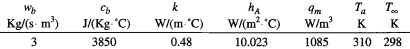
\includegraphics[width=15cm]{figuras/tabela.png}
\caption{Valores do parâmetros usados para análise Teórica. FONTE: \cite{Equacao}}.
\label{figura 3:Tabela}
\end{figure}

Portanto, a função se resume em:

\begin{gather}
373.081,77 (r-1)^5 - 7.481.688.555(r-1)^4 + 1.243.556,157(r-1)^3 \\
- 3.730.817,70 (r-1)^2 - 1.465.654,57(r-1)^2 - 253,793
\end{gather}

























